\documentclass[tikz, convert={convertexe=magick}, png]{standalone}

\usepackage[compat=0.4]{yquant}
\usepackage{braket}
\yquantset{register/default name=$\ket{\reg_{\idx}}$}
\usetikzlibrary{quotes}

\begin{document}
   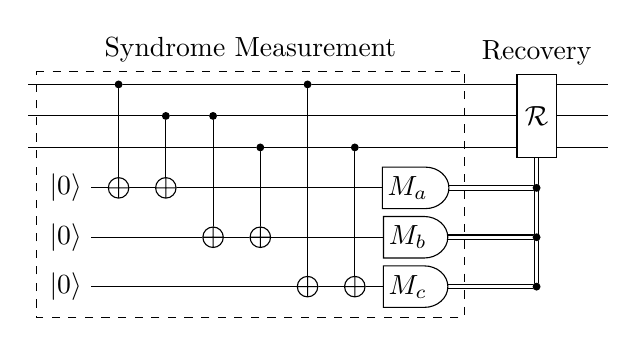
\begin{tikzpicture}
      \begin{yquant}
         qubit {} msg[3];
         nobit syndrome[3];
         
         [this subcircuit box style={dashed, "Syndrome Measurement"}]
         subcircuit {
            qubit {} msg[3];
            [out]
            qubit {$\ket0$} syndrome[3];
            
            cnot syndrome[0] | msg[0];
            cnot syndrome[0] | msg[1];
            cnot syndrome[1] | msg[1];
            cnot syndrome[1] | msg[2];
            cnot syndrome[2] | msg[0];
            cnot syndrome[2] | msg[2];
            
            dmeter {$M_{\symbol{\numexpr`a+\idx}}$} syndrome;
         } (msg[-2], syndrome[-2]);
         
         ["Recovery"]
         box {$\mathcal R$} (msg) | syndrome;
         discard syndrome;
      \end{yquant}
   \end{tikzpicture}
\end{document}